\section{Results and Discussion} \label{sec:results}

In this section, we report annotate-and-reconstruct experiments comparing phylogeny reconstruction quality obtained across possible hereditary stratigraphy approaches.
These experiments seek to establish an holistic, evidence-driven synopsis of each approach's suitability across experimental use cases.
The following section, ``A Practicioner's Guide to Hereditary Stratigraphy,'' then synthesizes findings to suggest guidelines for selecting appropriate methods to apply in practice.

This section delves into three primary aspects of hereditary stratigraphy methodology:
\begin{enumerate}
\item surface- versus column-based implementation,
\item tilted versus steady (versus hybrid) retention, and
\item bit- versus byte-sized differentiae.
\end{enumerate}

In a final set of experiments, we investigate how reconstruction quality fares with increasing phylogeny scale.
Scale-up of subsampled tip count and of underlying population size are both considered.
This question is crucial to application of hereditary stratigraphy for very large simulation use cases, in assessing the extent, if at all, annotation size would need to be boosted with increased experimental scale.

\subsection{Surface vs. Column} \label{sec:surface-vs-column}

\begin{figure*}
  \centering
  \begin{subfigure}[b]{0.5\textwidth}
    \centering
    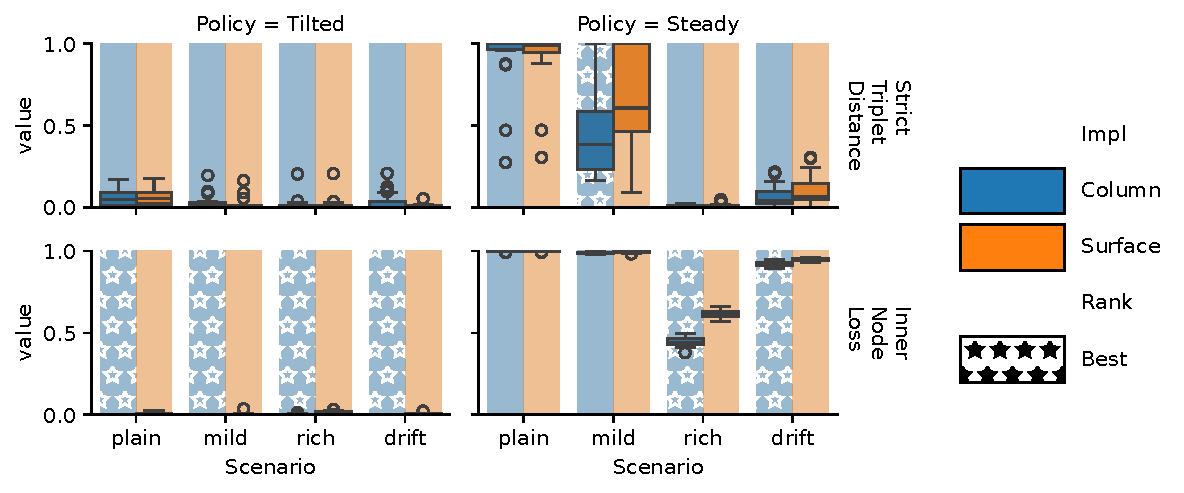
\includegraphics[width=\textwidth]{binder/binder/surf-vs-col/teeplots/annotation-size-bits=64+col=policy+differentia-width-bits=1+downsample=500+hue=impl+num-generations=100000+population-size=65536+post=teed-figure-subplots-adjust-right-0-72-teed-set-titles-row-templat.../e-row-name+row=variable+score=value+viz=peckplot+x=scenario+x-group=outer+y=value+ext=}
    \caption{Example reconstruction quality measure distributions. Lower is better.}
    \label{fig:col-vs-surf-example}
  \end{subfigure}%
  \begin{subfigure}[b]{0.5\textwidth}
    \centering
    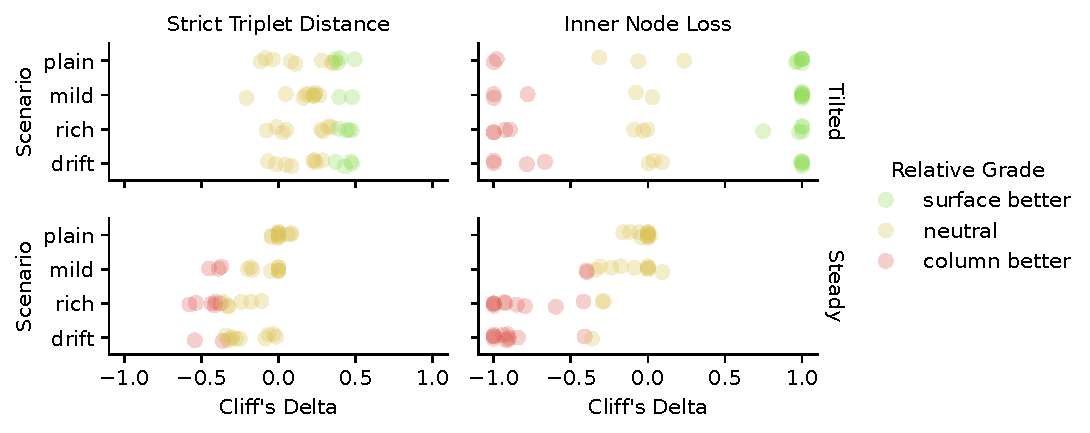
\includegraphics[width=\textwidth]{binder/binder/surf-vs-col/teeplots/col=metric+hue=relative-grade+kind=strip+post=teed-set-titles-col-template-col-name-row-template-row-name+row=policy+viz=catplot+x=cliff-s-delta+y=scenario+ext=}
    \caption{Reconstruction quality comparison outcomes.}
  \label{fig:col-vs-surf-overview}
  \end{subfigure}
  \caption{%
    \textbf{Does column- or surface-based instrumentation give higher-quality reconstruction?}
    Subpanel \ref{fig:col-vs-surf-overview} shows effect sizes of column-vs-surface comparisons for triplet distance and inner node loss metrics.
    Color coding indicates a significant outcome (Mann-Whitney U).
    Surface tends to outperform column under tilted policy and vice versa under steady policy.
    Subpanel \ref{fig:col-vs-surf-example} shows reconstruction quality effects for 64-bit size, bit-differentia annotations wit population size 65,536, downsample size 500, and 100k generations.
    Background hatching indicates significant outcome.
  }
  \label{fig:col-vs-surf-summary}
\end{figure*}


\begin{itemize}
    \item surf steady worse than col steady
    \item surf tilted better than col tilted
\end{itemize}

From this point onwards, only surf algorithms!!!

Figure \ref{fig:col-vs-surf-summary} compares reconstruction quality for surface algorithms against their corresponding column implementation.
We did this by using a simple simulation to generate phylogenies under different conditions with perfect tracking, then simulating heritage of hstrat annotations down the perfect tree and subsequent reconstruction.
We could then compare the reconstruction that would have been obtained under approximate tracking to the underlying ground truth.

To ensure generalizable results, we tested over a large number of evolutionary regimes, population sizes, instrumentation sizes, and instrumentation fingerprint sizes.
Each row in Figure \ref{fig:col-vs-surf} represents a distinct combination of surveyed conditions.

We took three measures of reconstruction quality.
The first measure, triplet distance, is a measure of accuracy --- it is the fraction of triplet tips that are correctly arranged in the reconstruction.
Whereas this metric considers polytomies as distinct from separate branching events, our second measure is a lax variant of triplet distance that does not penalize penalties introduced into the reconstruction (i.e., due to uncertainty about branching order) or over-resolution of true polytomies into more nodes in the reconstruction.
Finally, we also include inner node count, which provides a measure of the amount of detail achieved by reconstructions.
Higher inner node count indicates that fewer branching events are being lumped together into polytomies due to insufficient information to differentiate them.
This metric is only applicable to scenarios with fingerprint sizes larger than one bit (i.e., a byte), which are capable of generating non-bifurcating trees.

The data tell two clear stories:
\begin{enumerate}
\item surface tilted algorithms create higher-quality reconstructions than column-based tilted algorithms and
\item surface column algorithms create lower-quality reconstructions than column-based column algorithms.
\end{enumerate}

The surface tilted performs significantly best in 14 / 48 scenarios for triplet distance, 9 / 48 for lax triplet distance, and all scenarios where inner node count is applicable.
It performs significantly worse in no scenarios.

The surface steady performs significantly worse in 11 / 48 scenarios for triplet distance, in 1/48 scenarios for lax triplet distance, and 4/12 scenarios for inner node loss.
The surface steady performs significantly better than the column in no scenarios.

The performance advantage of surface-tilted is likely because the surface-based algorithms can make better use of available space --- every site is always in use to store a fingerprint.
In contrast, under the column-based approach, some fraction of the available space is typically unused because of difficulty predicting the order with which sites will need to be eliminated \textit{a priori} and thus eliminating them based on a heuristic (TODO rewrite this sentence).

The performance detriment of column-steady likely stems from precise control of the column approach to sequence eliminations.
The surface approach guarantees adherence to the fixed resolution qualities provided by the column approach, but the process of degrading from one spacing to the next double-width spacing is slightly more irregular on account of the additional consideration of being mapped onto the surface.
Unlike the tilted algorithm, the steady column algorithm does not have difficulty filling available space.

Recent work indicates that tilted policies should be preferred for better reconstruction accuracy in most cases, except where there are extreme factors promoting phylogenetic richness.
Thus, degraded reconstruction performance from the steady surface is not much of a concern because the steady policy is not expected to be used frequently in practice.
So, in addition to being capable of being implemented in a broader range of device contexts (not needing memory allocation or rich data structures) and being faster to calculate (discussed next), the surface-based approach can provide higher-quality phylogenetic reconstructions.

\subsection{Steady vs. Tilted} \label{sec:steady-vs-tilted}
\begin{itemize}
    \item steady worse than tilted
    \item hybrid similar to tilted
\end{itemize}

\begin{figure*}
  \centering
  \begin{subfigure}[b]{0.42\textwidth}
    \centering
    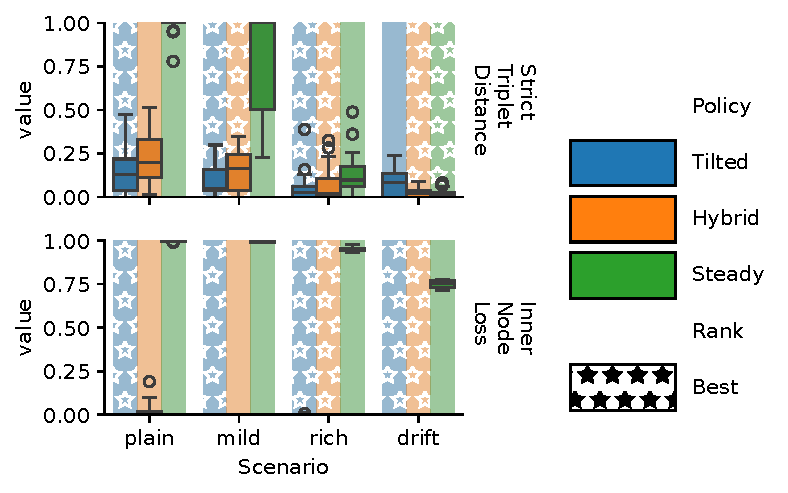
\includegraphics[width=\textwidth]{binder/binder/steady-vs-tilted/teeplots/annotation-size-bits=64+differentia-width-bits=1+downsample=500+hue=policy+num-generations=100000+population-size=65536+row=variable+score=value+viz=peckplot+x=scenario+x-group=outer+y=value+ext=}
    \caption{Example reconstruction quality distributions. Lower is better.}
    \label{fig:steady-vs-tilted-summary-example}
  \end{subfigure}%
  \begin{subfigure}[b]{0.58\textwidth}
    \centering
    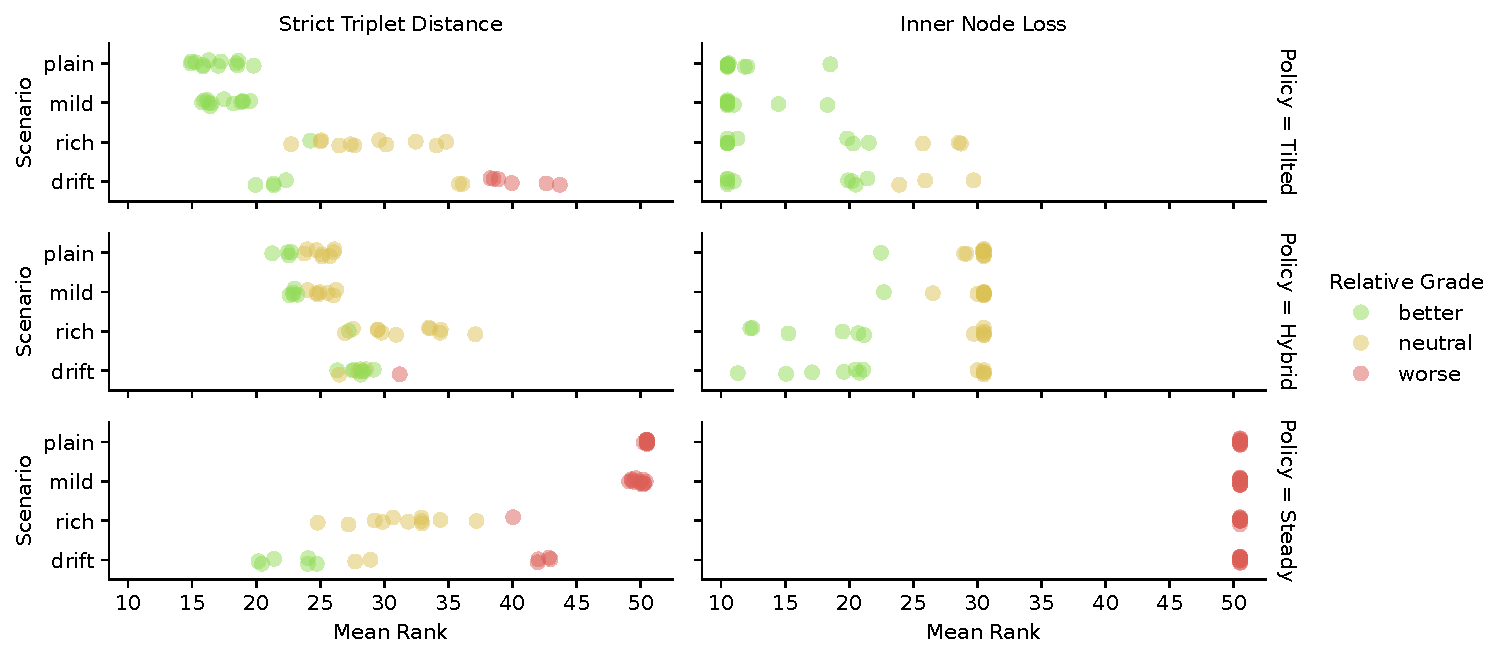
\includegraphics[width=\textwidth]{binder/binder/steady-vs-tilted/teeplots/col=metric+hue=relative-grade+kind=strip+row=policy+viz=catplot+x=mean-rank+y=scenario+ext=}
    \caption{Reconstruction quality comparison outcomes. Lower is better.}
    \label{fig:steady-vs-tilted-summary-overview}
  \end{subfigure}
  \caption{%
    \textbf{How does retention policy affect reconstruction quality?}
    \footnotesize
    Subpanel \ref{fig:steady-vs-tilted-summary-overview} shows mean rank among reconstruction error measures from tilted, hybrid, and steady retention policies across sensitivity analysis conditions.
    Each point represents an independent 20-replicate trial under different evolutionary conditions, instrumentation configuration (e.g., annotation size), and phylogenetic scale (e.g., reconstruction tip count).
    Color coding indicates significant outcome (Kruskal-Wallis H then Mann-Whitney U test).
    Lower is better.
    Tilted policy (top row) performs best in most evolutionary scenarios, except triplet distance under the highly phylogenetically-rich drift regime.
    Steady policy (bottom row) performs worst in most scenarios, except triplet distance under the drift regime.
    Hybrid policy performance has somewhat higher triplet distance reconstruction distance error in the plain and mild scenarios than tilted policy, but is robust to the drift regime.
    Subpanel \ref{fig:steady-vs-tilted-summary-example} shows reconstruction quality effects for 64-bit size, bit-differentia annotations with population size 65,536, downsample size 500, and 100k generations.
    Background hagching indicates significant outcome.
    See Supplementary Figure \ref{fig:steady-vs-tilted} for listing of reconstruction quality outcomes by sensitivity analysis condition \citep{moreno2024supplemental}.
  }
  \label{fig:steady-vs-tilted-summary}
\end{figure*}


\subsection{Why is Steady Bad? What Type of Error is Made?} \label{sec:error-analysis}
\begin{itemize}
    \item inner node loss from boxplot
    \item then, it's coming from recent nodes: node density vs. time histogram joyplot
    \item then, and that causes error: show error category (correct/wrong/unsure) vs. time stacked bar plot
\end{itemize}

From this point onwards, only surface-tilted (maybe also tilted-hybrid?) algorithm(s)!!!!

\subsection{Why are we seeing error? What can we do about it?} \label{sec:error-uncertainty}

mechanism of error: you have a lineage that diverges three ways between checkpoints (maybe make a figure of this); the two LEAST related happen to collide at the next checkpoint --- therefore, it looks like they're most related even though they're not.

sidebar: we can use differentia size to trade off between error and reconstruction accuracy; using 1 byte differentia essentially drives error to zero (but introduces uncertainty i.e., more polytomies in reconstruction)

\subsection{Differentia Width} \label{sec:bit-vs-byte}

\begin{figure*}
  \centering

\begin{minipage}{\textwidth}
\begin{subfigure}[b]{0.4\textwidth}
\centering
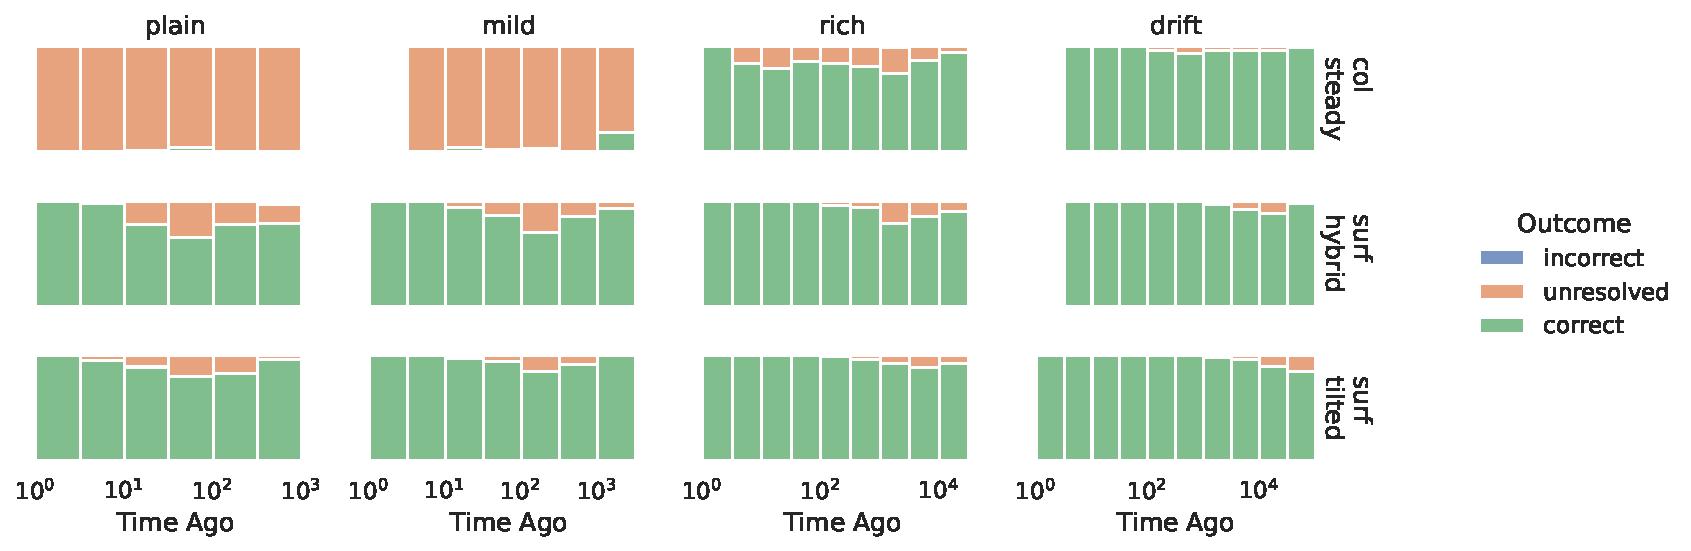
\includegraphics[height=1.2in,trim={0 0 5cm 0},clip]{binder/binder/teeplots/annotation-size=256+col=scenario+differentia-width=8+hue=outcome+kind=hist+multiple=fill+row=algo+scale=npop65536-ngen100000+viz=displot+x=time-ago+ext=}
\footnotesize
\caption{byte differentia outcomes; 256-bit annotation}
  \label{fig:bit-vs-byte-summary-byte-outcomes}
  \end{subfigure}%
\begin{subfigure}[b]{0.6\textwidth}
\centering
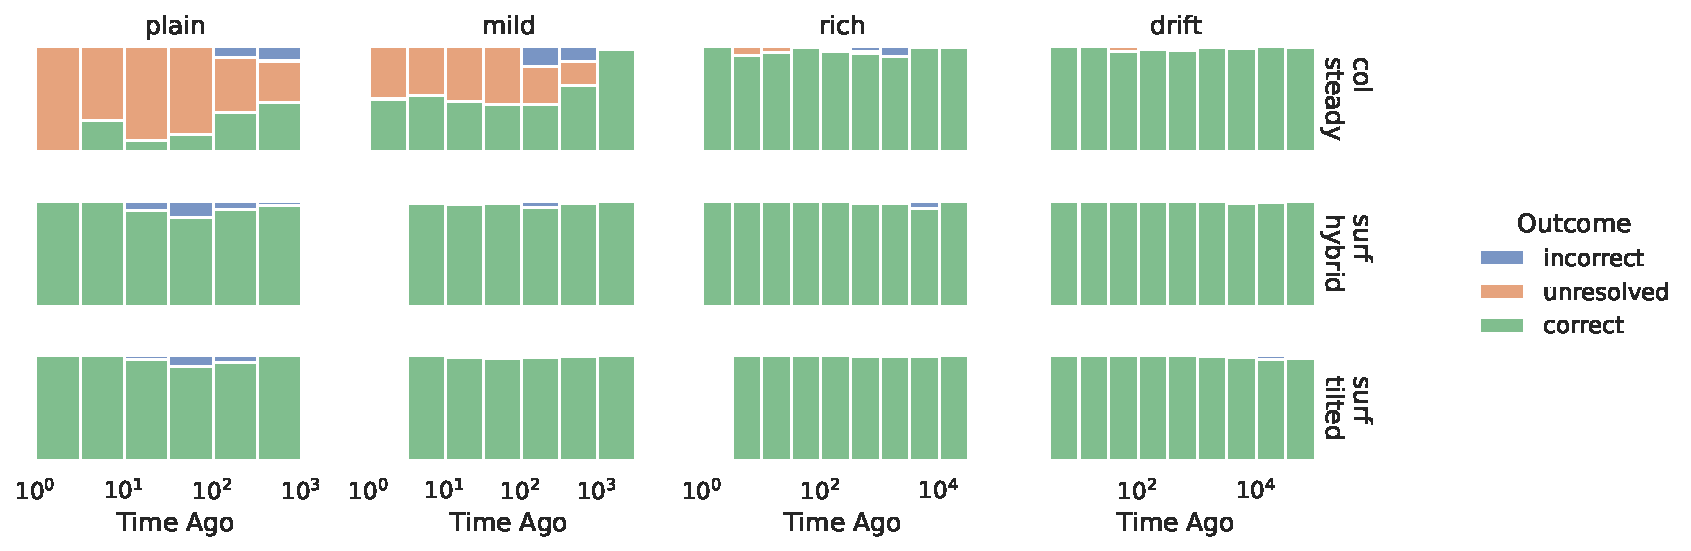
\includegraphics[height=1.2in]{binder/binder/teeplots/annotation-size=256+col=scenario+differentia-width=1+hue=outcome+kind=hist+multiple=fill+row=algo+scale=npop65536-ngen100000+viz=displot+x=time-ago+ext=}
\footnotesize
\caption{bit differentia outcomes; 256-bit annotation}
\label{fig:bit-vs-byte-summary-bit-outcomes}
\end{subfigure}
% \begin{subfigure}[b]{0.6\textwidth}
% \centering
% 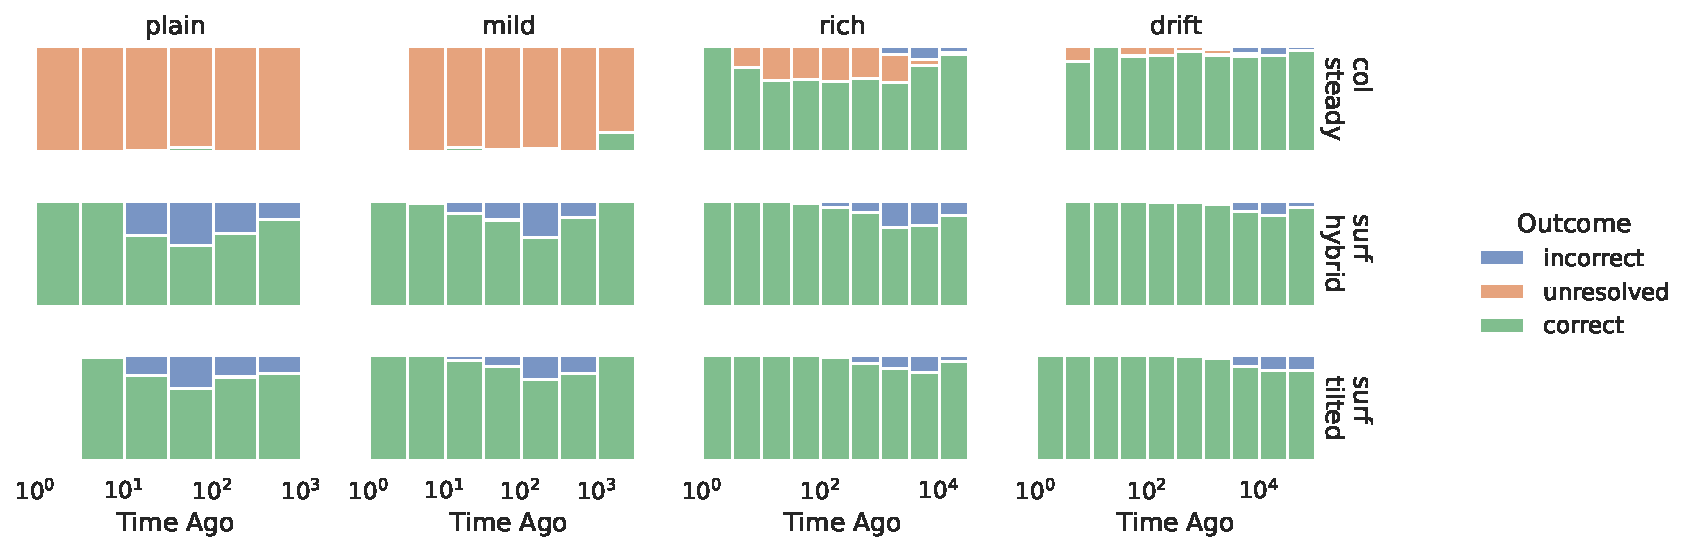
\includegraphics[height=1.2in]{binder/binder/teeplots/annotation-size=32+col=scenario+differentia-width=1+hue=outcome+kind=hist+multiple=fill+row=algo+scale=npop65536-ngen100000+viz=displot+x=time-ago+ext=}
% \caption{32-bit annotation, bit differentia}
% \end{subfigure}
\end{minipage}
% \begin{subfigure}[b]{0.4\textwidth}
%   \centering
%   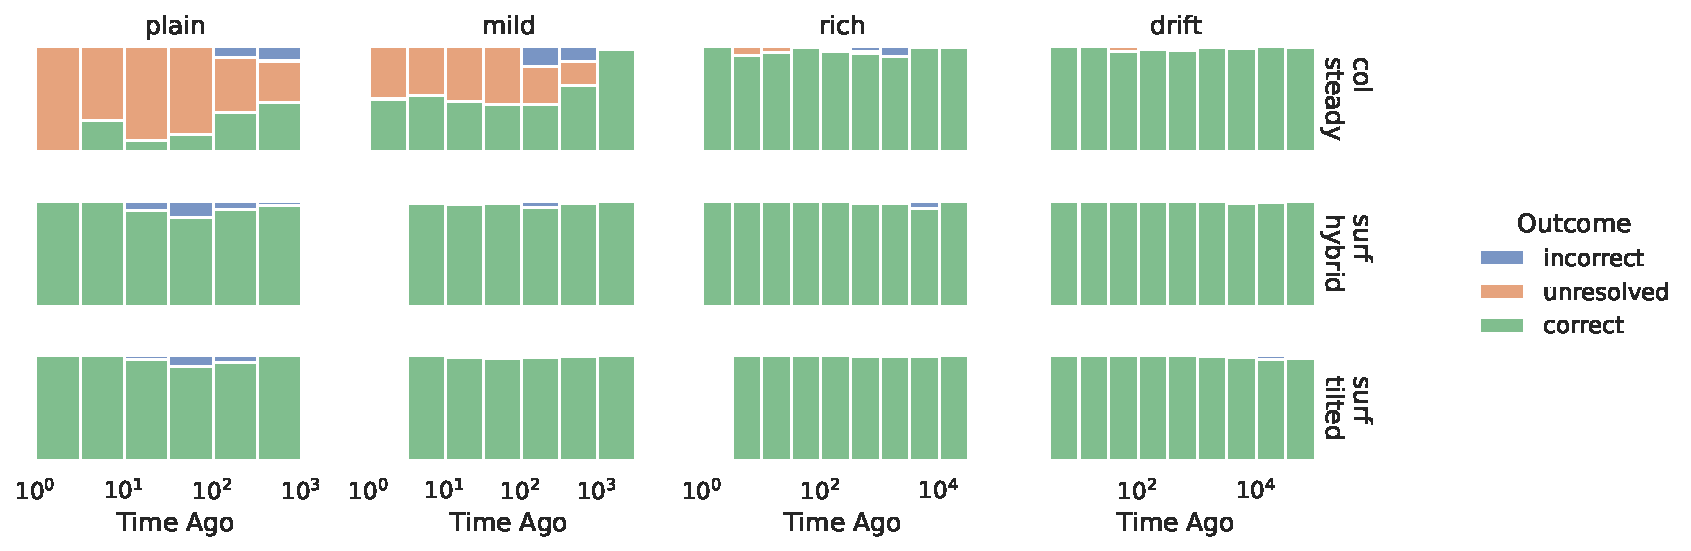
\includegraphics[height=1.2in,trim={0 0 5cm 0},clip]{binder/binder/teeplots/annotation-size=256+col=scenario+differentia-width=1+hue=outcome+kind=hist+multiple=fill+row=algo+scale=npop65536-ngen100000+viz=displot+x=time-ago+ext=}
%   \caption{reconstruction outcomes; 256-bit annotation, bit differentia}
%   \end{subfigure}%
  \begin{subfigure}[b]{\textwidth}
    \centering
    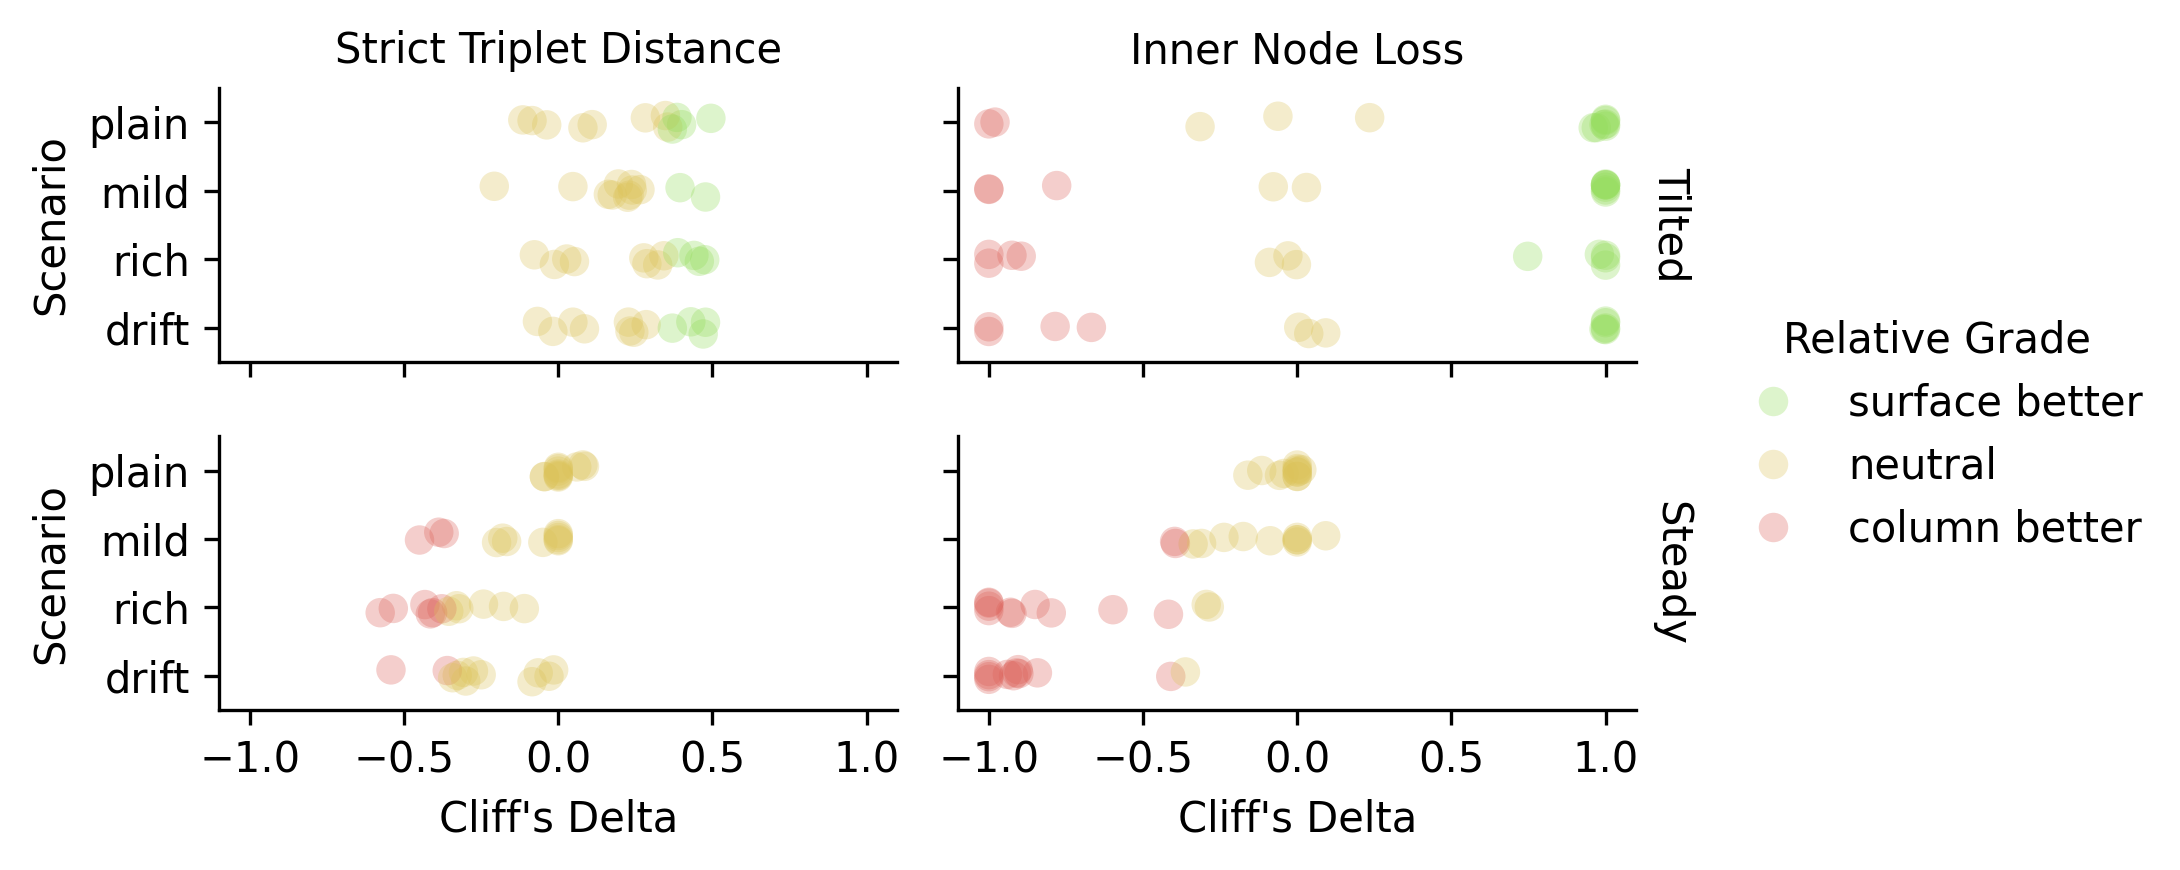
\includegraphics[width=0.8\linewidth]{binder/binder/bit-vs-byte/teeplots/col=metric+hue=relative-grade+kind=strip+row=policy+viz=catplot+x=cliff-s-delta+y=scenario+ext=}
    \footnotesize
    \caption{Reconstruction quality of byte differentia, relative to bit differentia; 256-bit size annotation}
  \label{fig:bit-vs-byte-summary-quality}
  \end{subfigure}%
\caption{%
  \textbf{How does differentia width affect reconstruction quality?}
  \footnotesize
   Top panels show reconstruction outcomes for phylogenetic branching events (Figure \ref{fig:hstrat-failure-modes}) under bit- and byte-width differentiae, respectively.
   Outcomes are binned by time ago (ranging from most recent to most ancient).
   Bottom panel compares reconstruction quality metrics between reconstructions from annotations with bit- and byte-width differentiae.
   Color coding indicates significance, with red indicating better bit-width differentia performance and green indicating better byte-width differentia performance.
   Byte-width differentiae consistently underperform bit-width differentia in inner node loss and strict triplet distance measures.
   However, byte-width differentiae outperform bit-width differentia in the lax triplet distance measure, which does not penalize polytomy triplets, i.e., isolating incorrect reconstruction from unresolved reconstruction (Figure \ref{fig:hstrat-failure-modes}).
  See Supplementary Figure \ref{fig:bit-vs-byte} for listing of effects by sensitivity analysis condition \citep{moreno2024supplemental}.
}
  \label{fig:bit-vs-byte-summary}

\end{figure*}


\subsection{Does it Scale?} \label{sec:scaling}
% https://tex.stackexchange.com/a/159294/316176
\newcommand{\rulesep}{\unskip\ \vrule\ }

\begin{figure*}
  \centering
  \begin{subfigure}[b]{0.33\textwidth}
    \centering
    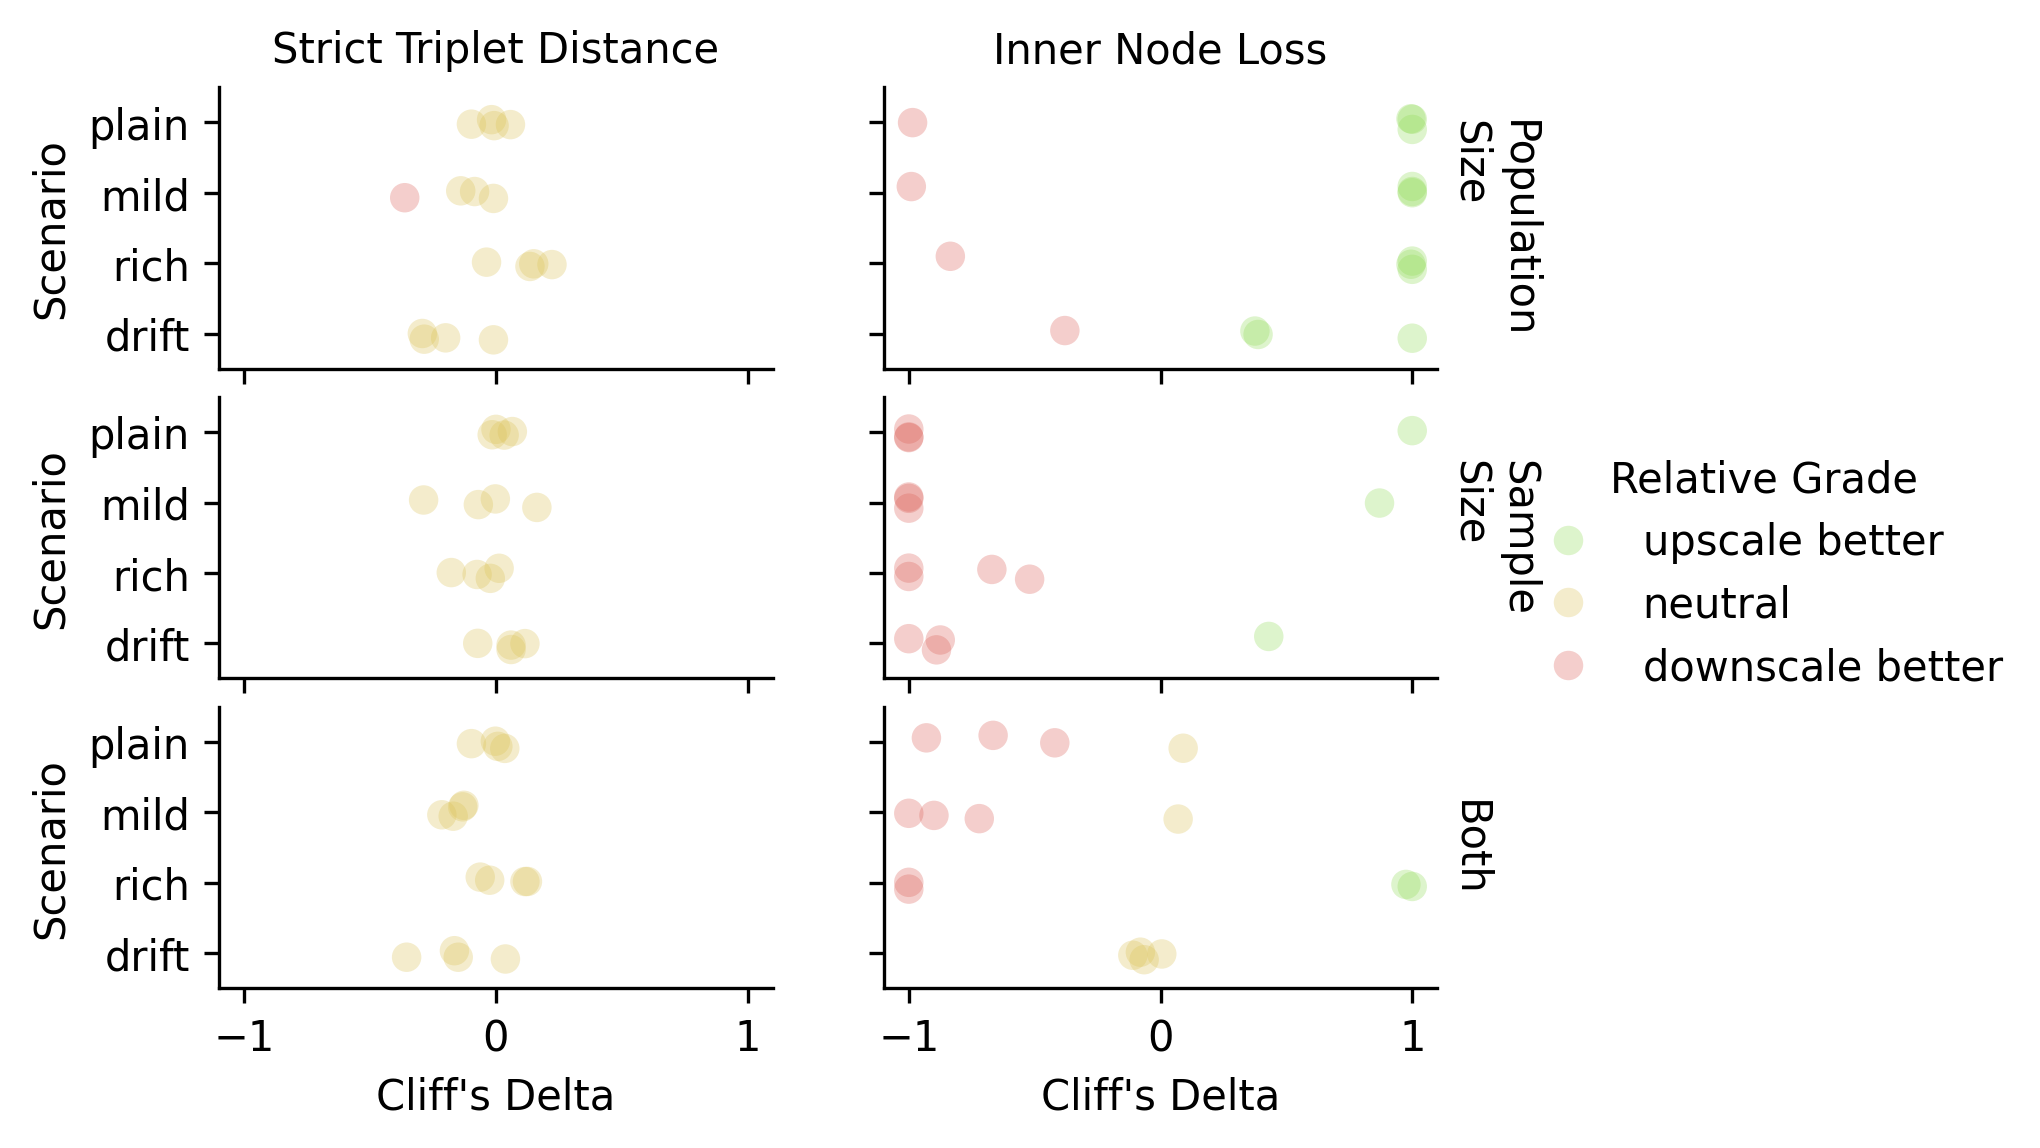
\includegraphics[height=1.7in,trim={0 0 5cm 0},clip]{binder/binder/dsamp-popsize-scale/teeplots/col=metric+hue=relative-grade+kind=strip+policy=tilted+row=scaling-factor+viz=catplot+x=cliff-s-delta+y=scenario+ext=}
    \caption{tilted retention policy (surface)}
  \end{subfigure}%
  \rulesep %
  \begin{subfigure}[b]{0.26\textwidth}
    \centering
    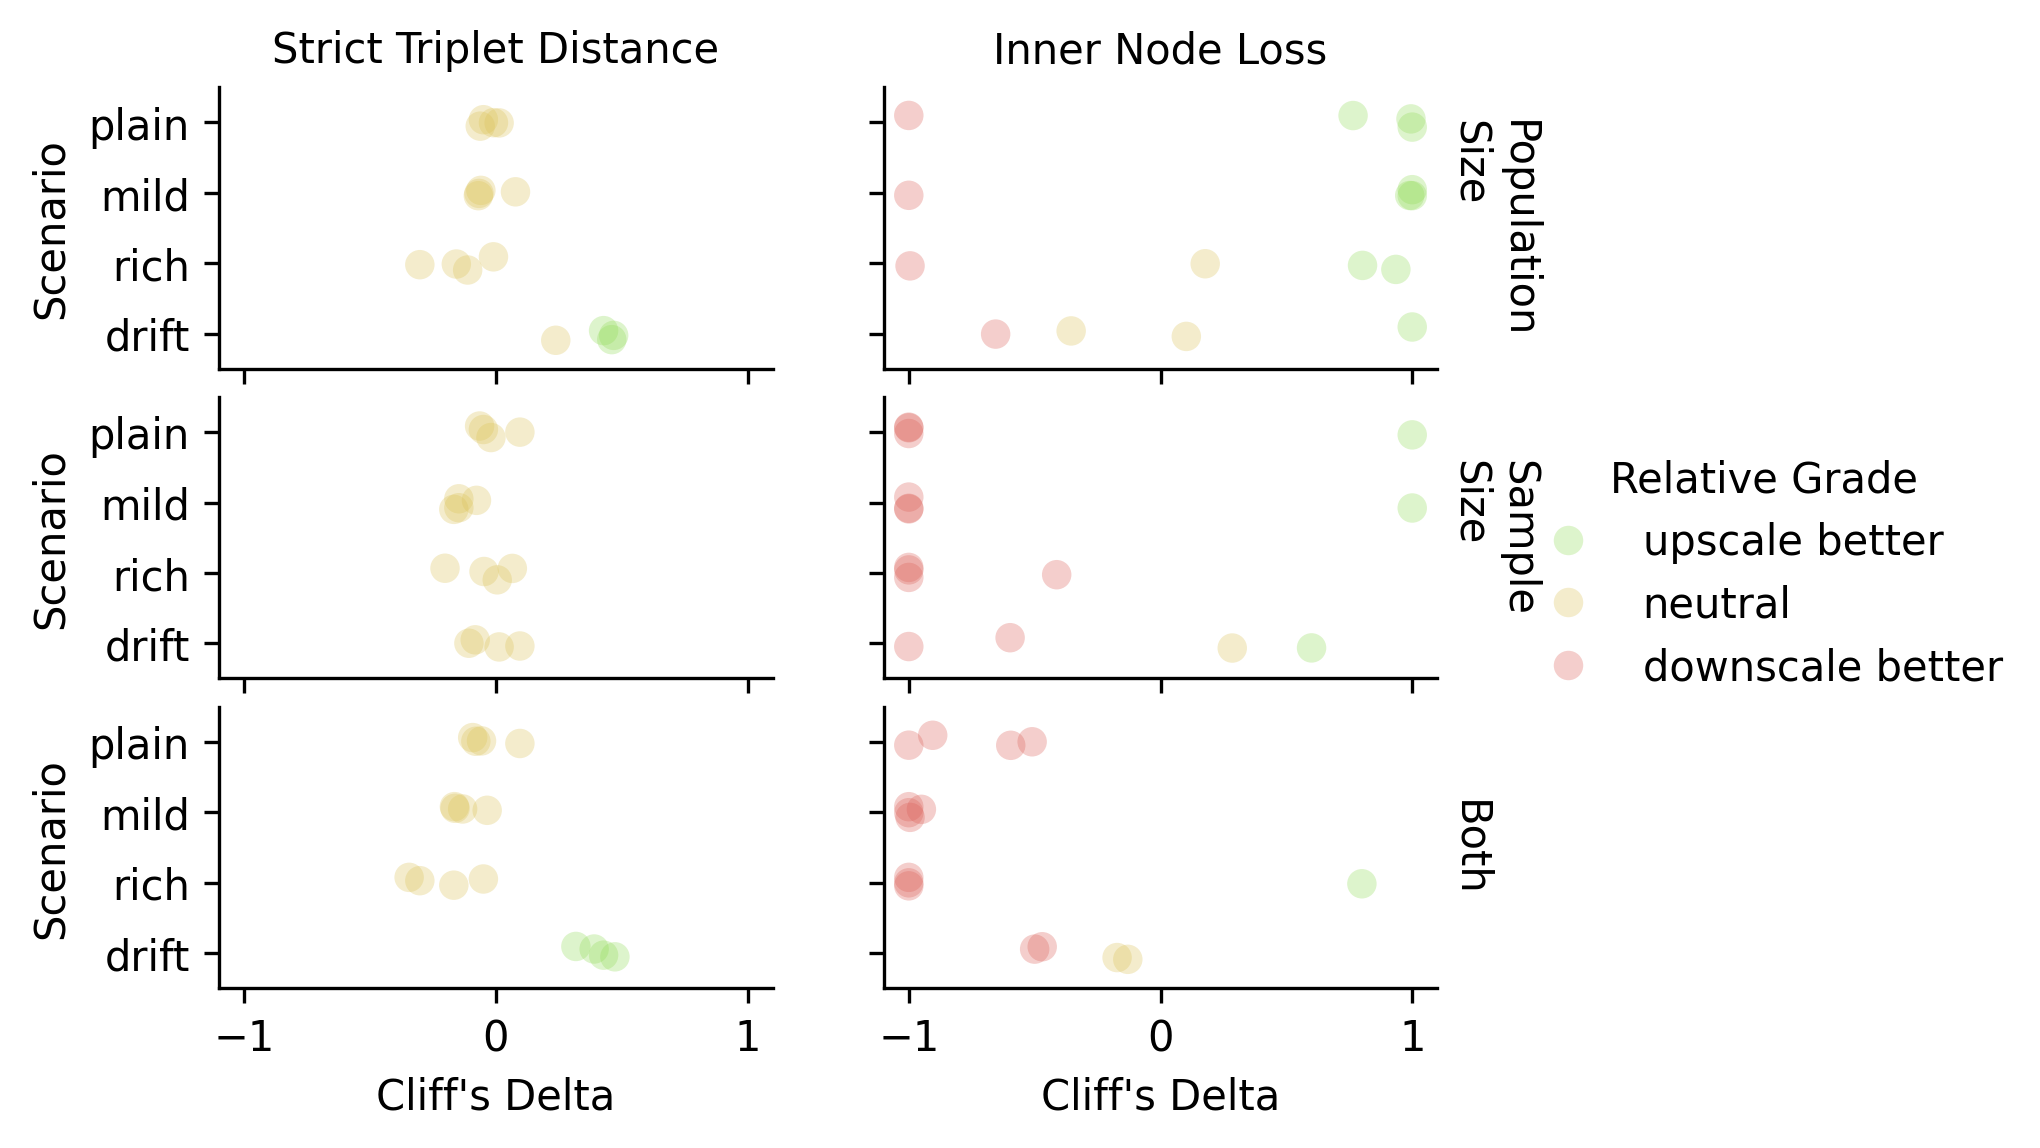
\includegraphics[height=1.7in,trim={2cm 0 5cm 0},clip]{binder/binder/dsamp-popsize-scale/teeplots/col=metric+hue=relative-grade+kind=strip+policy=hybrid+row=scaling-factor+viz=catplot+x=cliff-s-delta+y=scenario+ext=}
    \caption{hybrid retention policy (surface)}
  \end{subfigure}%
  \rulesep %
  \begin{subfigure}[b]{0.39\textwidth}
    \centering
    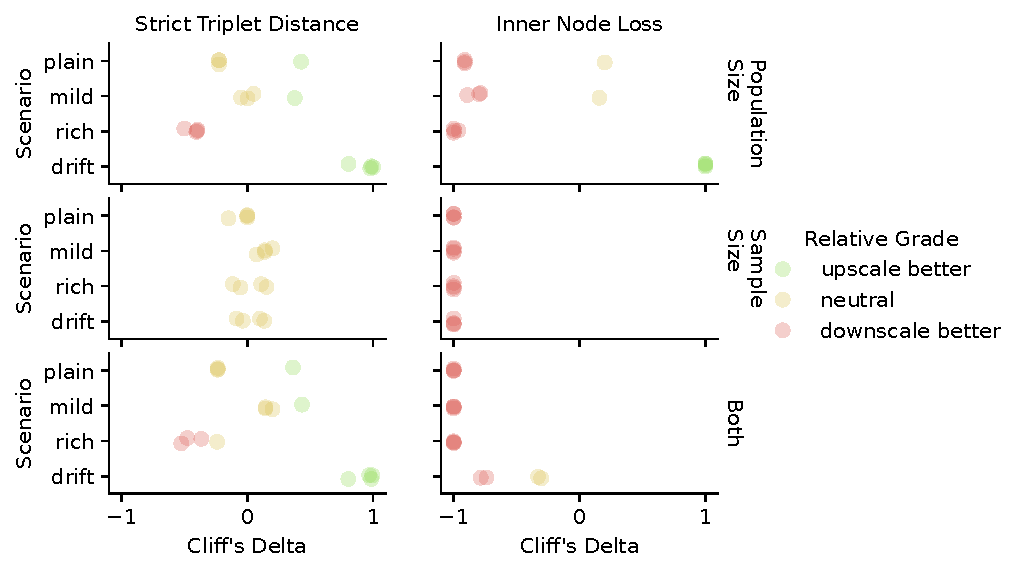
\includegraphics[height=1.7in,trim={2cm 0 0 0},clip]{binder/binder/dsamp-popsize-scale/teeplots/col=metric+hue=relative-grade+kind=strip+policy=steady+row=scaling-factor+viz=catplot+x=cliff-s-delta+y=scenario+ext=}
    \caption{steady retention policy (column)}
  \end{subfigure}
  \caption{%
  \textbf{How does scale impact reconstruction quality?}
  \footnotesize
  Each dot is a Cliff's Delta effect size of downscale-vs-upscale comparison under one sensitivity analysis condition.
  Color coding indicates a significant outcome (Mann-Whitney U).
  In order, rows show scaling outcomes for increasing population size, population subsample size (i.e., tree tip count), and both these factors.
  For tilted and hybrid policies, scaling had minimal effects on triplet distance and no systematic effect on inner node loss.
  Inner node loss worsened when scaling sample size, with and without scaling population size.
  Scaling effects were more variable under steady retention policy.
  See Supplementary Figures \labelcref{fig:dsamp-popsize-scale-hybrid,fig:dsamp-popsize-scale-steady,fig:dsamp-popsize-scale-tilted} for listing of effects by sensitivity analysis condition.
  }
  \label{fig:scaling-summary}
\end{figure*}


\begin{itemize}
    \item show reconstruction error and inner node count vs. pop size (error does not increase with pop size at fixed sample size)
    \item show reconst error/inner node count vs. time (error does not increase with time at fixed sample size)
    \item show reconst error/inner node count vs. sample size (error increases with sample size)
    \item show reconst error/inner node count vs. bit size at large sample (we can reduce the error for large sample size by increasing bit size)
\end{itemize}

Note that inner node loss will likely be less of an issue for asynchronous generations on account of leaves being generationally dispersed.
